\chapter{Experimentos e Resultados}
    \label{chap:resultados}
    
    Este capítulo apresenta como foram conduzidos os experimentos criados para avaliar a economia de energia obtida com o ambiente RT-DVFS construído. Os resultados destes experimentos são apresentados e analisados.
    
    \section{Ambiente Experimental}
    
        O ambiente experimental foi criado com base em um conjunto pré-definido de tarefas periódicas. Como métrica para avaliação, utilizou-se a potência média de todo o sistema, composto de uma placa-mãe Gumstix Connex e sua expansão HWUART, utilizada para transmissão de dados sobre RS232.
    
    \subsection{Tarefa Canônica}
    
        Para a avaliação, uma tarefa canônica foi concebida, cujo papel é comportar-se como uma tarefa de tempo real periódica. Sua escrita em C++ dá-se como uma função não-membro que recebe como argumento dois inteiros sem sinal. O primeiro representando a ocupação da tarefa, e um segundo, representando o número de invocações que a tarefa periódica receberá, conforme mostrado no texto em C++ \ref{tarefa-canonica}.
        
        \begin{lstlisting}[label=tarefa-canonica, escapeinside='', float=t, captionpos=b, caption=Exemplo de uma tarefa canonica como uma função não-membro]
        int cononical_task(unsgiend int busy, unsigned int iterations){
            
            for(unsigned int i = iterations; i > 0; i--){
                for(volatile unsigned int b = busy; b > 0; b--);
                EA_Periodic_Thread::wait_next();
            }
            
            return 0;
        }
        \end{lstlisting}
        
        A simulação da ocupação do processador pela tarefa nada mais é do que um laço vazio, que se repete por um número constante arbitrário de vezes. Para diferentes ocupações do processador, utiliza-se diferentes constantes para a repetição do laço. Esta abordagem é a mesma utilizada no trabalho de \citeonline{Lin:2010}, onde os autores propõem um \textit{framework} destinado à avaliação de heurísticas para RT-DVFS. Vale salientar que a tarefa apresentada simula tarefas \textit{CPU-bound}, ou seja, tarefas que tem seu tempo de execução limitado principalmente pela frequência da CPU, utilizando poucas instruções que fazem acesso à memória principal.
        
    \subsection{Aplicações EPOS para Experimentação}
    
        Utilizando-se então a tarefa canônica, cinco aplicações para o sistema EPOS foram criadas, cada uma composta por três tarefas periódicas (utilizando=se a abstração \emph{EA\_Periodic\_Thread}) baseadas na tarefa canônica apresentada. As aplicações foram elaboradas para simularem 100, 80, 60, 40 e 20\% de ocupação total de CPU, sempre considerando um acréscimo de 5\% na ocupação total como sobrecarga do próprio sistema operacional e tempo de alteração de tensão e frequência para o processador. Isto significa que, uma aplicação que simula 100\% de uso, na realidade utiliza 95\% do tempo de CPU com suas tarefas. Concluindo, para uma utilização $u$, cada pior tempo de computação $C'_i$ utilizado na aplicação é na realidade $C'_i=(u-0,05u)C_i$.
        
        Para se conseguir o número de repetições do laço de cada tarefa canônica, constantes foram empiricamente aplicadas pelo programador. Utilizando-se o método \emph{cc} da abstração \emph{EA\_Periodic\_Thread}, que por sua vez utiliza o TSC do sistema, foi calculada a utilização de cada tarefa. As constantes assumidas para experimentação passaram por 10 sessões de execução por 5 segundos em configuração de frequência máxima, onde a utilização esperada pelo programador foi atingida com um desvio padrão menor que 0.01\% da média amostral. O pior tempo de computação, passado como parâmetro para a criação de cada \emph{EA\_Periodic\_Thread}, foi extraído como o maior tempo de computação obtido da amostragem citada.
        
        Cada uma das aplicações cria um conjunto de três tarefas periódicas, estas com 500, 400 e 300 milisegundos de período. A aplicação indica um número de repetições para cada tarefa, de modo que elas se repitam durante pelo menos 305 segundos. A interrupção do \emph{timer} de sistema do EPOS foi reduzido para um período de 100 milisegundos, sendo compatível com os períodos das tarefas apresentadas.
        
        Do conjunto de configurações para tensão e frequência apresentados na tabela \ref{tab:configuracoes}, o subconjunto mostrado na tabela \ref{tab:configuracoes-utilizadas} foi utilizado. Os critérios para a escolha destas configurações foram:
        
        \begin{itemize}
            \item Não há variação na frequência da memória principal, comportamento que não será avaliado neste trabalho.
            \item Para todos dispositivos que variam a frequência, o subconjunto oferece uma ordem total dos elementos (hipótese necessária para o funcionamento das heurísticas implementadas).
            \item Uniformidade (cada frequência do núcleo é um múltiplo aproximado de 0,25, ou seja, conforme a teoria apresentada na seção \ref{sec:escalonamento-em-sistemas-rt-dvfs}, há $\alpha$ 0,25, 0,50, 0,75 e 1,00).
        \end{itemize}
        
        \begin{table}
        \begin{tabularx}{\textwidth}{ |C|C|C|C| }
            \hline
            Tensão do processador ($V$)&
            Frequência do Núcleo ($MHz$)&
            Frequência do PXBus ($MHz$)&
            Frequência da SDRAM ($MHz$)\\ \hline \hline
            $1.0$ & $99,5$ & $50,0$ & $99,5$ \\ \hline
            $1.0$ & $199,1$ & $99,5$ & $99,5$ \\ \hline
            $1.1$ & $298,6$ & $99,5$ & $99,5$ \\ \hline
            $1.3$ & $398,1$ & $186,0$ & $99,5$ \\ \hline
        \end{tabularx}
        \captionof{table}{Configurações de tensão e frequência do PXA255 utilizadas nos experimentos}
        \label{tab:configuracoes-utilizadas}
        \end{table}
        
        As caches de dados e de instruções foram desligadas para a realização dos experimentos.
        
    \subsection{Configuração para Medições}
    
        Para a realização das medições, a placa Connex foi devidamente ligada à sua fonte de corrente contínua. Em seu circuito de alimentação, um resistor de 1$\Omega$ com 1\% de variação foi colocado em série com o cabo da fonte, assim como mostrado pela figura \ref{fig:setup}.
        
        \begin{figure}[h]
        \begin{center}
        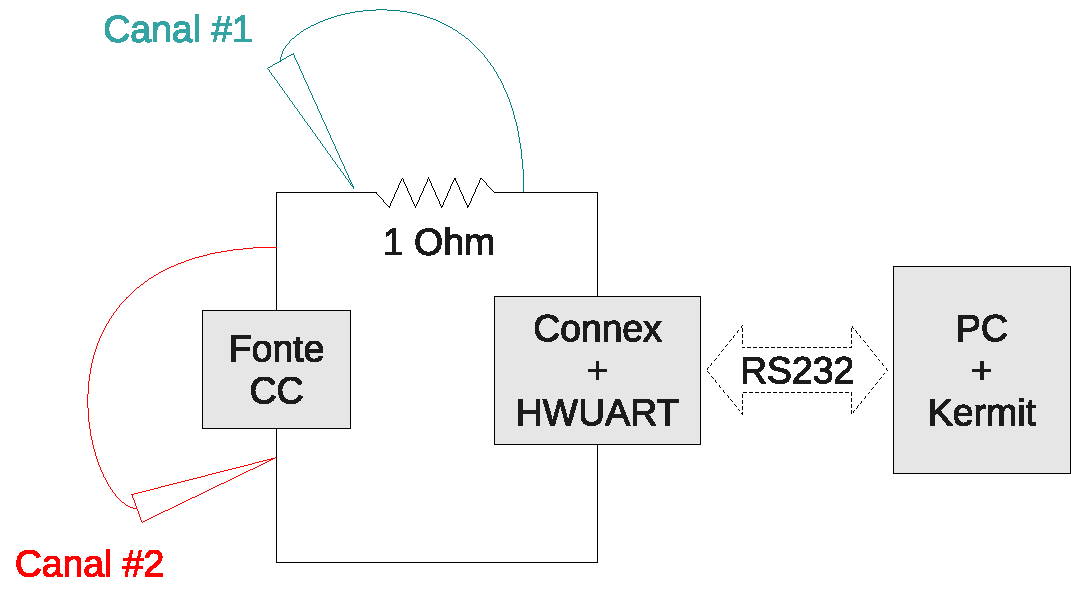
\includegraphics[scale=0.6]{imagens/setup.pdf}
        \captionof{figure}{Configuração do experimento utilizado para medições}
        \label{fig:setup}
        \end{center}
        \end{figure}
        
        Utilizando-se os canais de um osciloscópio digital, dois pontos do circuito de alimentação foram amostrados a $5Hz$: a queda de tensão no resistor apresentado e a tensão na fonte de alimentação, conforme a figura \ref{fig:setup}.
        
        A tensão medida entre as pontas do resistor, pela Lei de Ohm, pode ser convertida na corrente aproximada que passa pelo circuito. Através dessa corrente $I$ e a tensão da fonte de alimentação $U$, pode-se então ser calculada em um instante a potência $P$ dissipada pelo sistema, esta sendo $P=U\cdot I$.
        
        Para a avaliação dos resultados, a potência média $P_{med}$ foi escolhida como métrica. Sendo $U(t)$ e $I(t)$, respectivamente, a tensão e corrente do sistema no instante $t$, pode-se calcular a potência média de um instante $0$ até $T$ como sendo: $$P_{med}={1\over T}\cdot \int_{0}^{T}U(t)\cdot I(t) dt.$$
        
        A escolha da potência média como métrica deve-se ao fato de ela representar, substancialmente, o trabalho elétrico realizado por todo o dispositivo (placa-mãe e expansão). Devido à alta granularidade temporal dos eventos, a sumarização através da média não traz prejuízo à leitura do comportamento das heurísticas.
        
        Para a transmissão das aplicações à placa Connex, essa foi ligada a um PC utilizando-se o padrão RS232.
        
        \subsection{Coleta e Compilação dos Dados}
        
        As aplicações de teste foram carregadas utilizando-se a facilidade Kermit do U-Boot, como já relatado no capítulo \ref{chap:desenvolvimento}. A coleta das amostras adquiridas pelo osciloscópio foi feita através de um ``\textit{pendrive}'', no qual é possível gravar as leituras obtidas. Um programa escrito na linguagem Python foi desenvolvido com o fim de processar as amostras contidas no pendrive, calculando então a potência média utilizada para a execução das aplicações.
        
        Para cada aplicação, repetiu-se 5 vezes o processo de carregamento em memória e execução do sistema. A potência média foi calculada para estas 5 amostras, o desvio padrão manteve-se sempre entre 1\% e 2\% da potência média. Os resultados obtidos são apresentados e discutidos na seção seguinte (\ref{sec:resultados}).
    
    \section{Resultados}
        \label{sec:resultados}
        
        O gráfico apresentado na figura \ref{fig:100-100}, mostra a potência média obtida para uma utilização real igual à utilização de pior caso, ou seja, o caso onde a utilização real por cada tarefa é igual à utilização referente ao pior tempo de computação passado como parâmetro para a construção do objeto \emph{EA\_Periodic\_Thread}.
        
        \begin{figure}[h]
        \begin{center}
        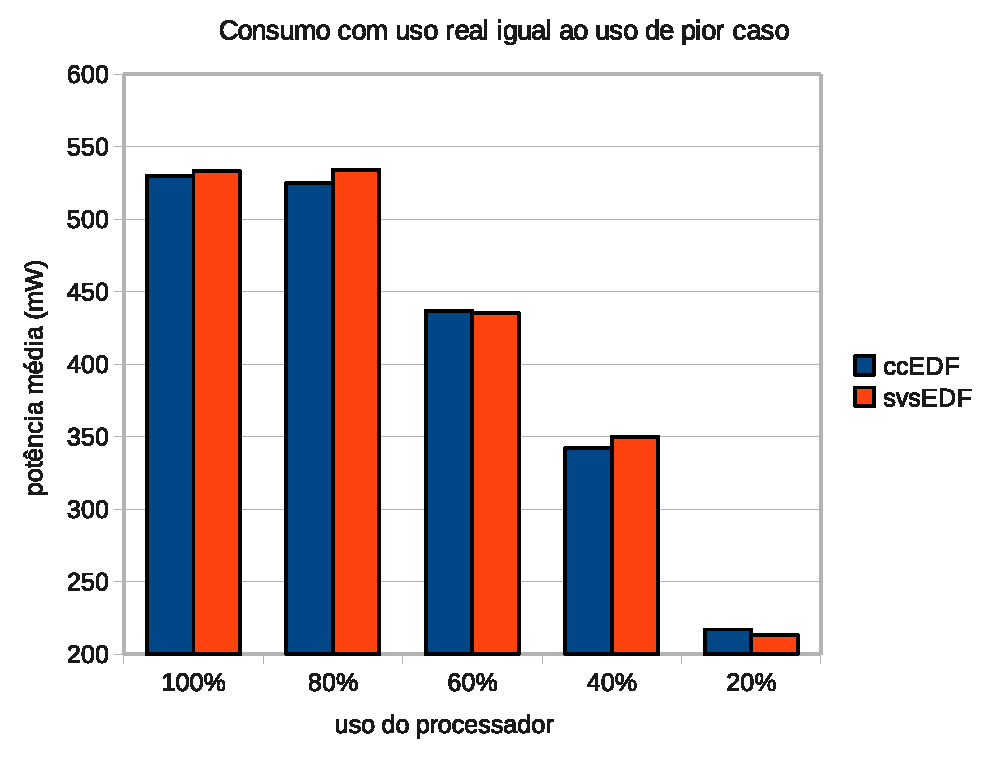
\includegraphics[scale=0.7]{imagens/grafico-100-100.pdf}
        \captionof{figure}{Gráfico da potência média com utilização real igual a de pior caso}
        \label{fig:100-100}
        \end{center}
        \end{figure}
        
        Observe que para as duas heurísticas implementadas, tanto \emph{Cycle-conserving} (ccEDF) como para \emph{Static Voltage Scaling} (svsEDF), não existe diferencial significativo no consumo entre os dois mecanismos. Isso se dá porque a heurística ccEDF tende a comportar-se como a heurística svsEDF quando a utilização real e de pior caso estão muito próximas, já que o resultado do cálculo estático e dinâmico da utilização neste caso são equivalentes. A pequena variação entre o consumo das duas heurísticas nos mesmos casos ocupação acontece devida a erros experimentais e à pequena variação presente na utilização real das tarefas.
        
        Ainda, o gráfico da figura \ref{fig:100-100} é capaz de mostrar diretamente os efeitos que as configurações de tensão e frequência causam no consumo de energia total do sistema, já que neste caso as duas heurísticas são equivalentes. A tabela \ref{tab:efeitos} apresenta a possível relação entre o uso de processador e a configuração selecionada pelo heurística estática svsEDF, segundo o que é apresentado no gráfico. Há variação na potência média para frequência normalizada 1,00 devido a erros experimentais.
        
        \begin{table}[h]
        \begin{tabularx}{\textwidth}{ |C|C|C|C|C| }
            \hline
        		Uso & Frequência de CPU & Frequência normalizada & Tensão   & Potência média \\ \hline \hline
        		$100\%$ & $398,1MHz$ & $1,00$ & $1.3V$ & $533mW$ \\ \hline   
           		$80\%$ & $398,1MHz$ & $1,00$ & $1.3V$ & $534mW$ \\ \hline
           		$60\%$ & $298,6MHz$ & $0,75$ & $1.1V$ & $435mW$ \\ \hline           		
           		$40\%$ & $199,1MHz$ & $0,50$ & $1.0V$ & $350mW$ \\ \hline
           		$20\%$ & $99,5MHz$ & $0,25$ & $1.0V$ & $213mW$ \\ \hline
        \end{tabularx}
        \captionof{table}{Relação entre uso de processador e configurações de tensão e frequência utilizadas}
        \label{tab:efeitos}
        \end{table}
        
        % É interessante observar que, mesmo não havendo queda de tensão entre os casos de 20 e 40\% de utilização, ainda há ganho energético. Teoricamente, a troca entre as configurações correspondentes a 0,25 e 0,50 de desempenho não deveria ser energeticamente eficiente. Neste experimento, acredita-se que a obtenção deste resultado é devida à redução da frequência do dispositivo PXBus, que provavelmente não oferece limites às tarefas em execução.
        
        O gráfico apresentado na figura \ref{fig:100-variando} mostra o comportamento das heurísticas com utilização de pior caso total, mas apresentando uma variação na utilização real entre 20 e 100\%. Isto significa que, mesmo as tarefas tendo como parâmetro um pior tempo de computação que causa 100\% de utilização, na realidade as tarefa canônicas correspondentes realizam apenas uma porcentagem fixa de 20 a 100\% do pior caso de computação. 

        \begin{figure}[h]
        \begin{center}
        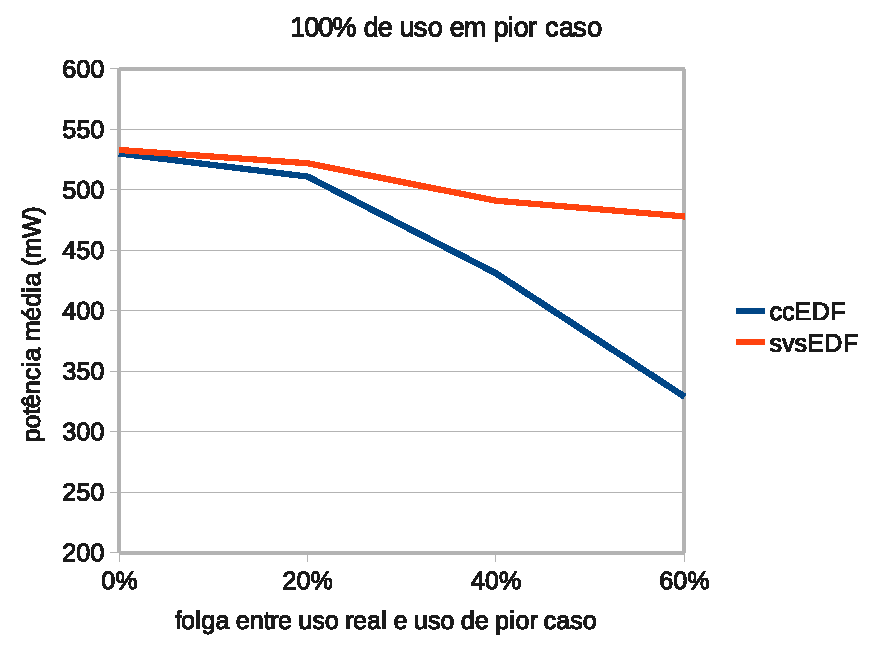
\includegraphics[scale=0.6]{imagens/100-variando.pdf}
        \captionof{figure}{Potência média em 100\% de uso de pior caso do processador com variação no uso real}
        \label{fig:100-variando}
        \end{center}
        \end{figure}
        
        A variação na utilização real apresentada demonstra a atuação da heurística dinâmica ccEDF, que leva em conta dados obtidos durante a execução do sistema. Observe que as curvas são muito próximas até a utilização real de 80\%, efeito causado pela indisponibilidade de uma configuração de tensão e frequência que represente um desempenho entre 0,75 e 1,00. O ganho só se torna observável a partir de 60\% de uso real, onde a heurística ccEDF calcula o uso dinâmico inferior ao de pior caso obtido estaticamente. A economia apresentada pela heurística estática é devido à redução no uso físico de componentes do circuito do processador.
        
        Observe que, no funcionamento da heurística dinâmica, o pior tempo de computação configurado estaticamente para cada tarefa quase sempre elevará a utilização calculada dinamicamente. O caso onde isto não acontece é quando todas tarefas foram completadas, sabendo-se o tempo de computação real utilizado por cada uma. De qualquer modo, na forma como a heurística ccEDF é escrita, este valor é ``sujado'' com o pior caso em novas requisições de tarefas. Aqui encontra-se a principal limitação da heurística \emph{Cycle-conserving}. É este tipo de problema que heurísticas de previsão (citadas na subseção \ref{sec:escalonamento-em-sistemas-rt-dvfs}) tentam resolver.
        
        \begin{figure}[h!]
        \centering
        \subfloat[]{
        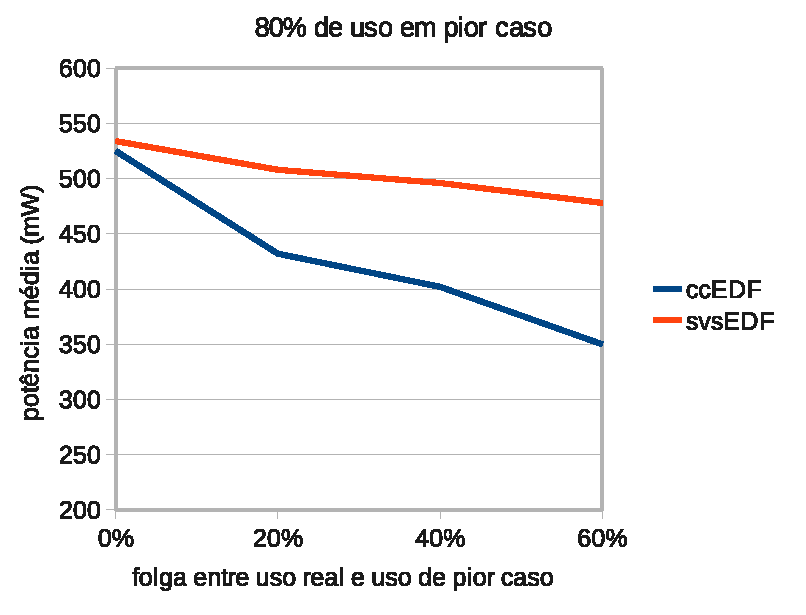
\includegraphics[scale=0.5]{imagens/grafico-80-variando.pdf}
        \label{fig:80-variando}
        }
        \subfloat[]{
        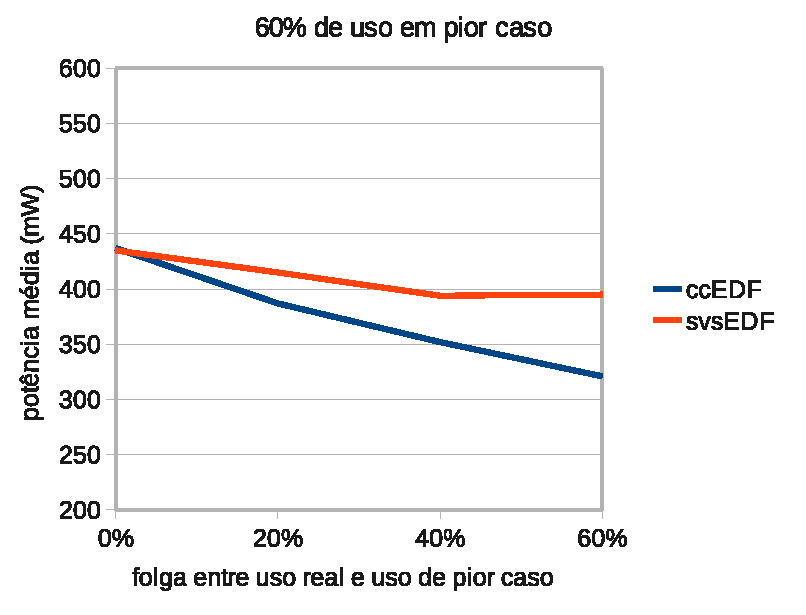
\includegraphics[scale=0.5]{imagens/grafico-60-variando.pdf}
        \label{fig:60-variando}
        }\\
        \subfloat[]{
        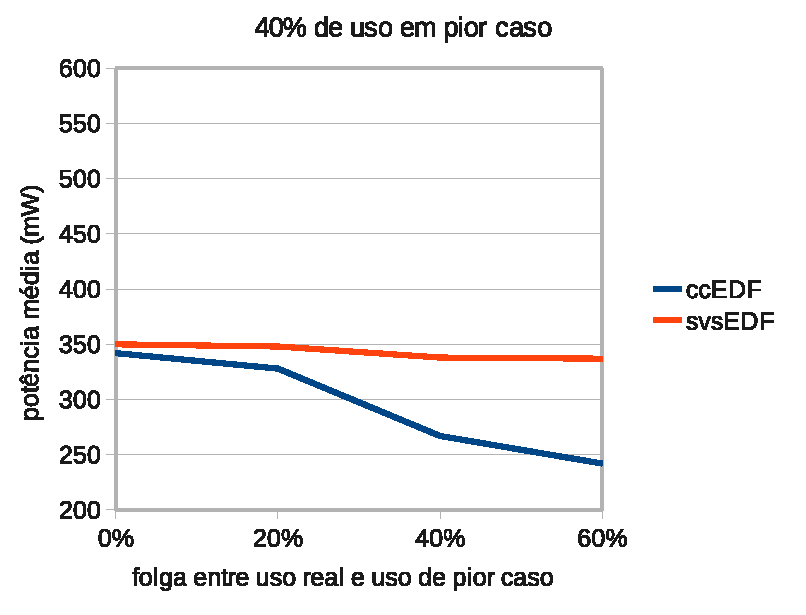
\includegraphics[scale=0.5]{imagens/grafico-40-variando.pdf}
        \label{fig:40-variando}
        }
        \subfloat[]{
        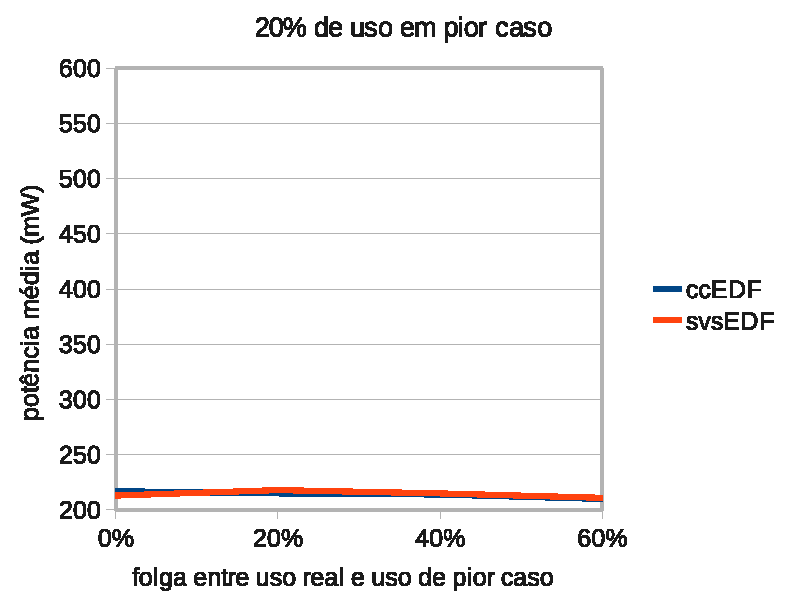
\includegraphics[scale=0.5]{imagens/grafico-20-variando.pdf}
        \label{fig:20-variando}
        }
        \caption{Potência média para uso de pior caso de 20 a 80\% com variação no uso real}
        \label{fig:80-20}
        \end{figure}
        
        O comportamento para outras utilizações de pior caso e variações no uso real, pode ser visualizado na figura \ref{fig:80-20}. É possível observar, novamente, uma queda no consumo utilizando-se a heurística svsEDF (itens \ref{fig:80-variando}, \ref{fig:60-variando}, \ref{fig:40-variando} e \ref{fig:20-variando}) isto se dá devido à redução no uso do processador. É interessante salientar que esta queda tende-se a estabilizar com redução do uso, como pode-se observar em \ref{fig:20-variando}. Isto acontece porque em d, a maior influência no consumo total do sistema passa a ser a energia estática consumida pelo PXA255, ou seja, a energia consumida não referente às consecutivas trocas de estado do circuito digital. 
        
        Ainda sobre \ref{fig:20-variando}, devido à baixa granularidade das configurações de frequência utilizadas, não há configurações de desempenho tão inferior sendo utilizadas para uso do processador inferior a 25\%, a heurística ccEDF não causa nenhuma influência.
        
        O sistema colocado em questão utilizando a heurística svsEDF pode ser entendido como um sistema de tempo real padrão com escalonamento EDF. Pode-se observar que mesmo não sendo ótima, a heurística ccEDF ainda obtém ganhos de até 25\% (na figura \ref{fig:80-variando}) neste cenário, e sem a perda de prazos. De qualquer modo, vale salientar que estes resultados sofreriam modificações caso as heurísticas fossem expostas em aplicações reais. Primeiramente, é imaginável que a folga entre uso real e de pior caso seria uma variável estocástica, como é de se esperar neste tipo de sistema. Em segundo, aplicações reais tendem a fazer um uso maior dos componentes do processador. Fatores importantes, como a influência da habilitação da memória cache do processador e aplicação de DVFS na SDRAM do PXA255 são temas para pesquisa futura.
